\subsection{UC11 - Visualizzazione risultato ricerca scaffalatura}
\begin{figure}[H]
  \centering
  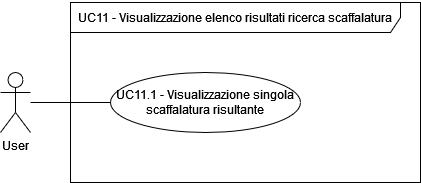
\includegraphics[width=0.8\textwidth]{UC_diagrams_11-20/UC11.drawio.png}
   \caption{Diagramma UML UC11}
\end{figure}
\begin{itemize}
    \item \textbf{Attori:} User.
    \item \textbf{Pre-condizione:} L'utente ha ricercato una scaffalatura [UC10].
    \item \textbf{Post-condizione:} La scaffalatura risultante dalla ricerca viene selezionata [UC8].
    \item \textbf{Scenario Principale:} L'utente, dopo aver ricercato un determinato codice, visualizza la scaffalatura corrispondente che verrà automaticamente selezionata.
    \item \textbf{Generalizzazioni:} -
    \item \textbf{Estensioni:} -
\end{itemize}